\documentclass[a4paper, 12pt]{article}

\usepackage{float}
\usepackage[T1]{fontenc}
\usepackage[utf8]{inputenc}
\usepackage[swedish]{babel}
\usepackage{graphicx}
\usepackage{natbib} % ger Harvard-referenser
\usepackage{graphicx}
\usepackage{listings}
\usepackage{color}

\setlength{\parskip}{12pt}
\setlength{\parindent}{0pt}


\begin{document}
    \title{Haskell in Javascript}
    \author{
        Adam Bengtsson, 
        Mikael Bung, 
        Johan Gustafsson, 
        Mattis Jeppsson 
        \\ 
        Institutionen för data- och informationsteknik 
        \\ 
        Chalmers Tekniska Högskola 
        \\ 
        41296 Göteborg
    }
    \date{\today}
    \maketitle
    \thispagestyle{empty}
    \newpage
    

\begin{abstract}
  Detta är en kort sammanfattning av innehållet i rapporten. Detta
  brukar kallas för \emph{sammanfattning} på svenska och
  \emph{abstract} på engelska.
\end{abstract}

    \thispagestyle{empty}
    \newpage
    \renewcommand{\abstractname}{Abstract}
    \begin{abstract}
Haskell is not a widely used programming language, nor very known to the average programmer. By implementing a subset of the Haskell 98 specification in Javascript our intention is to make it  possible to run Haskell in a web browser, thus making it easier for beginners to try Haskell by eliminating the need of downloading Haskell compilers such as GHC. 
\\
\\
In this paper we describe the process and result from the project of implementing Haskell in Javascript. 
Our result consists of a parser, type checker, interpreter and a front end similar to GHCi.
The parser process the text input, creating an internal structure called abstract syntax tree (AST). The type checker then analyse the AST to confirm that there are no type errors. If no errors have been detected, the AST is sent to the interpreter. The interpreter then interpret the AST in an well defined way.
\\
\\
The results shows that it's possible to successfully implement Haskell in Javascript,  but a lot of more work need to be done for making a newbie-friendly environment for learning Haskell. 

    \end{abstract}

    \thispagestyle{empty}
    \newpage

    \thispagestyle{empty}
    \tableofcontents
    \thispagestyle{empty}
    \thispagestyle{empty}
    \newpage

    \listoffigures
    \thispagestyle{empty}
    % include all parts
    \newpage
 %   \section{Förord}
TODO: Här tackar vi de som på ett eller annat sätt
hjälpt oss med projektet...

 %   \newpage
 %   \section{Förkortningslista}
TODO:kanske ej behövs??

 %   \newpage
    \section{Inledning}
\subsection{Bakgrund och motivation}
På vissa av Chalmers och Göteborgs Universitets datorvetenskapliga program är den första programmeringskursen i Haskell \citep{haskell98} och för en del av de nya eleverna är inlärningströskeln hög. De studenter som börjar på de datavetenskapliga programmen på Chalmers och Göteborgs Universitet är allt från nybörjare till mycket kompetenta inom programmering. De flesta saknar dock kunskaper kring funktionell programmering. Skillnaden mellan ett funktionellt och ett objektorienterat programmeringsspråk är stora och omställningen hur programmeringsrelaterade problem behöver angripas  är inte enkelt för de flesta nybörjare. Vi tror att ett interaktivt webbverktyg skulle kunna sänka tröskeln och underlätta undervisningen. Ett webbverktyg medför även att extra verktyg som Glasgow Haskell Compiler \citep{ghc} ej behövs installeras. Webbens stöd för interaktivitet gör det möjligt att snabbt visa funktionsdeklarationerna för de inbyggda funktionerna och att enkelt evaluera funktionerna och testa sig fram till olika resultat.

Många programmerare kommer inte i kontakt med funktionell programmering  och med hjälp av ett interaktivt webbbverktyg som är enkelt för användaren att använda är vår förhoppning att fler programmerare och studenter ska komma i kontakt med funktionell programmering, och i synnerhet Haskell. Då flera moderna objektorienterade programmeringsspråk börjar ta funktionalitet och begrepp från funktionella programmeringsspråk så är det extra viktigt att programmerare kommer i kontakt med funktionell programmering. Ett exempel på detta är C\# som i senare versioner har fått stöd för bland annat lambdafunktioner \citep{csharp}. 

En fördel med att ha tolken på webben är att det enda som behövs för att använda den är en javascriptkompatibel webbläsare, något som följer med i princip i alla moderna operativsystem. Detta betyder att de användare som befinner sig inom vår målgrupp redan har den programvaran som behövs på sina hemdatorer för att använda sig av vårt program.  
Haskell är ett starkt statiskt typcheckat och funktionellt programmeringsspråk med lat evaluering. % TODO: Citera, skriv om ifall det är direktöversatt
% jag bytte från strikt semantik till lat evaluering:p
Att språket är funktionellt innebär bland annat att funktioner är \emph{first-class citizens} och kan därmed användas som parametrar och returneras från andra funktioner precis som vilken annan typ som helst.

Lat evaluering innebär mer konkret att evalueringen av ett uttryck inte kommer utföras förrän resultatet av uttrycket behövs. Om uttrycket inte behövs  kommer interpretatorn att ignorera det. 
Lat evaluering gör att programmeraren inte behöver bry sig om exekveringsordningen av ett program. Detta ger prestandaförbättringar eftersom ett uttryck inte evalueras alls om det inte behövs \citep{hudak89}.
Lat evaluering gör det också möjligt att använda sig av oändliga datastrukturer, till exempel oändliga listor. Språket blir därmed mer uttrycksfullt. 

%Funktionella programmeringsspråk såsom Haskell anses också vara det naturliga steget att ta när man vill nå en högre abstraktionsnivå än den som imperativa programmeringsspråk tillåter. % TODO: citera
John Hughes argumenterar för att  funktionella språk som stödjer lat evaluering erbjuder större möjligheter än imperativa språk att skriva modulära program. Detta för att funktionella språk som Haskell stödjer higher order functions och lat evaluering vilket är tekniker som kan användas för att binda samman olika moduler.
Dessa två programspråksegenskaper bidrar till att program skrivna i Haskell är generellt sätt kortare och går fortare att skriva än motsvarande program skrivet i ett imperativt programmeringsspråk  \citep{why}.

Med ovan nämnda resonemang ser vi det som ovärderligt för programmerare att komma i kontakt och lära sig funktionell programmering. 
Förhoppningen är att vår Haskelltolk i Javascript ska kunna användas som grund för att i framtiden göra en interaktiv läroplattform för nybörjare i funktionell programmering. 


\subsection{Syfte}
Syftet är en implementera en fungerande Haskelltolk i Javascript. Den ska kunna tolka en delmängd av Haskell-specifikationen så den kan användas för att göra exempelvis interaktiva tutorials för nybörjare.
Meningen är att dessa ska kunna köras i en vanlig webbläsare utan att ladda ner en Haskellkompilator, till exempel GHC, eller behöva lära sig svårbegripliga kommandon.

\subsection{Problembeskrivning} 
%% WHAT THE FACK SKA VI SKRIVE HEAR?!!Ö!

\subsection{Metod}
Projektet består av planera, designa och implementera haskelltolken. Vi arbetade efter en iterativ modell där nya funktioner lades till undan för undan. Detta fungerar bra eftersom vi får en tidigt fungerande prototyp att utgå från. Arbetet delades upp i separata moduler som utvecklades relativt frånskillt från varandra för att undan för undan fasas ihop till det slutgiltliga resultatet. 

%I vårt arbete har vi implementerat parser, typcheckare och interpretator parallellt med varandra och utökar de olika modulernas funktionalitet iterativt.
%Vi hade tänkt följa den här planen genom varje milstolpe genom att utöka parsern, typcheckaren och interpretatorn med ny funktionalitet.

%Ett första delmål är att göra en enkel implementation av lambda calculus då mer avancerade funktionella programspråksegenskaper kan implementeras som detta \citep{jones87}.
% Parsern implementeras med hjälp av ett parser combinator bibliotek kallat JSParse \citep{jsparse}. Detta ger oss möjlighet att att på ett enkelt sätt implementera både den kontextfria och icke kontextfria delen av Haskell. Parsern skapar ett syntaxträd som skickas vidare till typcheckaren. I typcheckaren dekoreras syntaxträdet med typinformation innan det slutligen skickas till interpretatorn.

%Vi använder även JSParse, en parser combinator, för att bygga ett syntaxträd som skickas till typcheckaren och interpretatorn. I typcheckaren dekoreras syntaxträdet med typinformation.

%En interaktiv kommandotolk som kan köras i en webbläsare kommer att utvecklas. Den ska ge användaren möjlighet att skriva Haskell-funktioner och exekvera dem på ett liknande sätt som i GHCi. 
%Vi kommer att integrera jQuery \citep{jquery} för att få ett unisont stöd för samtliga webbläsare. jQuery kommer även underlätta arbetet med att skapa ett enkelt och stilrent interaktivt gränssnitt.

\subsubsection{Avgränsningar} 
Att tolka Haskell i Javascript är inget trivialt projekt och därför kommer inte hela Haskell att implementeras. Vi kommer implementera en delmängd av den version av Haskell som kallas Haskell 98.
De delar som prioriteras är
        \begin{enumerate}
            \item{Lambda-funktioner, namngivna funktioner}
            \item{Typer, generella typer, algebraiska datatyper}
            \item{Typklasser}
            \item{Pattern matching}
            \item{Guards}
        \end{enumerate}
Med dessa delar implementerade kan de flesta enklare Haskellprogram köras och bör vara tillräckligt för det stora flertalet nybörjare. Vi kommer ej lägga någon tid på att skapa en användarvänlig webbsida utan fokus kommer ligga på att skapa Haskelltolken. Dock kommer en kommandotolk som körs på en webbsida utvecklas för att kunna kommunicera med Haskelltolken. 
Vi kommer inte lägga någon nämnvärd tid på att optimera Haskelltolken utan målet är att göra en fungerande implementation. 


    \setcounter{page}{10}
    \newpage
    \section{Teori}

    \newpage
    \section{Metod} 

Nedan följer en beskrivning av de arbetsmetoder, mjukvaror och kodbibliotek som vi använt oss av i projektet. 

\subsection{Genomförande}

% modulbaserat arbete..
För att implementera en tolk för Haskell behövs en parser för den aktuella syntaxen, en typcheckare för språkets definerade typregler och tillsist en interpretator som tolkar språket efter dess specifikation.
Det upptäcktes tidigt att de tre modulerna, parser, interpretator och typcheckare inte behövde utvecklas sekvensiellt. De tre modulerna intergrerar enbart med varandra genom det abstrakta syntaxträdet, vår interna representation av Haskell, vilket medför att det är lätt att utveckla de olika modulerna helt frånskilt från varandra. Figur \ref{fig:tolkens_struktur} visar hur denna interaktion mellan de olika modulerna är tänkt att gå till. Figuren visar även hur webbläsaren kommunicerar genom ett Javascript API och det abstrakta syntaxträdet och inte direkt med de olika komponenterna. 

\begin{figure}[h]
    \begin{center}
        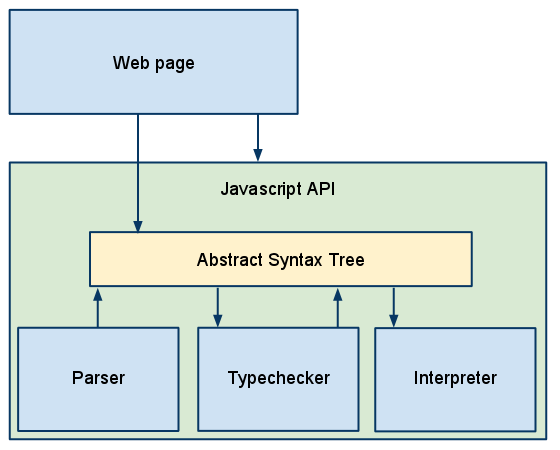
\includegraphics[width=1.0\textwidth]{image1.png}
        \caption{Överblick över tolkens struktur och interaktion}
        \label{fig:tolkens_struktur} % Labels must come after caption!
    \end{center}
\end{figure}

Det första delmålet var att göra en haskelliknande implementation av lambda calculus då mer avancerade funktionella programspråksegenskaper kan implementeras som detta \citep{jones87}.
Parsern implementerades med hjälp av ett \emph{parser combinator}-bibliotek kallat JSParse \citep{jsparse}. Det gav oss möjlighet att på ett enkelt sätt implementera både den kontextfria och icke kontextfria delen av Haskell. Parsern skapar ett syntaxträd som skickas vidare till typcheckaren. I typcheckaren dekoreras syntaxträdet med typinformation innan det slutligen skickas till interpretatorn.

En interaktiv kommandotolk som kan köras i en webbläsare utvecklades. Den gav användaren möjlighet att skriva haskellfunktioner och exekvera dem på ett liknande sätt som i GHCi. 
Vi integrerade jQuery \citep{jquery} för att få ett unisont stöd för samtliga webbläsare. jQuery underlättade även arbetet med att skapa ett enkelt och stilrent interaktivt gränssnitt.

Arbetssättet präglades av en iterativ utvecklingsmetodik med korta utvecklingscyklar. Arbetet delades upp med huvudansvarstagande över var sin modul och utfördes parallellt med varandra. Arbetet skedde dock framförallt i samlad grupp på grund av att det var många designrelaterade problem vi var tvugna att ta ställning till under projektet, till exempel hur vårat abstrakta syntaxträd skulle se ut, och för att det skulle bli enklare när vi skulle börja sammanfoga våra olika moduler med varandra. 
Det var också ett bra sätt att snabbt få hjälp av varandra eftersom vi ej visste exakt hur modulerna skulle se ut när vi påbörjade arbetet. Vi fann det därför praktiskt att använde en iterativ modell för att bit för bit utvigda våra moduler. Dock valde vi att implementera typcheckaren i ett steg då vi ansåg att det skulle vara enklare. Detta främst för att vi trodde typklasser var så centralt i typcheckaren att det skulle vara svårt att lägga till det i en andra iteration. 

Eftersom vi arbetade parallellt med olika moduler var vi beroende av ett bra versionshanteringssystem. Bra i vårt fall innebar att det skulle vara enkelt att arbeta i olika grenar, en gren för varje modul, och att det skulle gå snabbt och enkelt att slå ihop dessa förgreningar när vi behövde länka samman två utvecklares arbeten. I början av projektet använda vi oss av Subversion (SVN). Detta berodde framförallt på att det var det versionshanteringssystem som alla i gruppen hade erfarenhet från tidigare. Dock insåg vi att SVN inte var praktiskt att använda när man arbetar i flera olika grenar i projektet samtidigt. Därför gick valet till att använda Git som är designat från grunden för att på ett enkelt sätt skapa nya och slå samman förgreningar under utvecklingens gång. Vi kunde därmed skapa en förgrening för varje modul och under arbetets gång sammanlänka allas arbeten på ett effektivt sätt. 

På grund av vår parallella arbetsmetod ansåg vi det nödvändigt att arbeta fram en kodstandard så att de olika modulerna skulle stilmässigt likna varandra. Kodstandarden beskriver hur indentering och namngivning av variabler och funktioner ska se ut. Innan ny kod skickades till Git så krävdes det att koden uppfyllde kraven i kodstandarden.  

%\subsection{Javascript} 
%Javascript \citep{javascript} är ett programmeringsspråk som framförallt används på klientsidan på webben. Javascript är ett dynamiskt objektorienterat skriptspråk.
%Javascript är det programmeringsspråk som används uteslutande i detta projektet.

\subsection{Kodbibliotek}
I projektet använder vi oss av tre kodbibliotek för att snabbare kunna utveckla haskelltolken. Nedan följer en kort beskrivning av dessa.

\subsubsection{JSParse}  
Parsern implementeras med hjälp av ett parser combinator bibliotek kallat JSParse. 
En parser combinator består av olika funktioner som parsar exempelvis strängar, listor eller blanksteg.
Dessa funktioner kombineras för att skapa mer komplexa parsers. Det ger oss möjlighet att implementera komplexa
parsers för både de kontextfria och icke kontextfria varianterna av Haskell.

\subsubsection{jQuery} 
%jQuery är ett öppet kodbibliotek till Javascript som är dubeellicenserat under MIT License och GPL version 2.  
jQuery är designat för att underlätta för utvecklare att modifiera DOM-träd och göra asynkrona javascript-anrop. jQuery användes i projektet för att få likartat stöd i samtliga webbläsare i kommandotolken som utvecklades. 
jQuery gav oss även möjlighet att skapa ett enkelt och stilrent interaktivt gränssnitt utan att behöva göra allt från grunden.
jQuery.Cookie, ett tillägg till jQuery, används för att förenkla användandet av kakor.

\subsubsection{JSON}
JSON \citep{json}  är en delmängd av Javascript och används för att utbyta data mellan olika format och programmeringsspråk. 
JSON är idag inbyggt i de senaste versionerna av de moderna webbläsarna, men för att få stöd i äldre versioner har vi valt att inkludera JSON som ett externt bibliotek.


    \newpage
    \section{Resultat}
% TODO

Projektets resultat är ett kodbibliotek för en haskelltolk. Här presenterar vi de olika modulerna som tolken består av. Koden finns att tillgå på GitHub: \url{http://github.com/johang88/haskellinjavascript}.

\subsection{Parser} 
Parserns uppgift är att ta användarens indata och konvertera den till en datastruktur 
som är lättare att hantera internt. Denna datastruktur kallas Abstract Syntax Tree (AST). 
Haskellstandarden har definerat upp en grammatik, ett antal regler, som definerar hur korrekt haskellkod ser ut och hur den ska tolkas.

För att parsa indatan använder vi ett bibliotek för att bygga parsers, kallat JSParse \citep{jsparse}.
JSParse ger oss ett antal funktioner som vi använder för att definera grammatiken och konvetera den till vår interna struktur.

Som figur \ref{fig:parser_steg} visar, så består parsern av tre mindre parsers, den första är en parser som hittar kommentarer och tar bort dessa. 
Den andra identifierar haskellkod som inte är kontextfri och gör om till kontextfri kod. Den tredje gör om den kontextfria koden till vår AST.

\begin{figure}[H]
    \begin{center}
        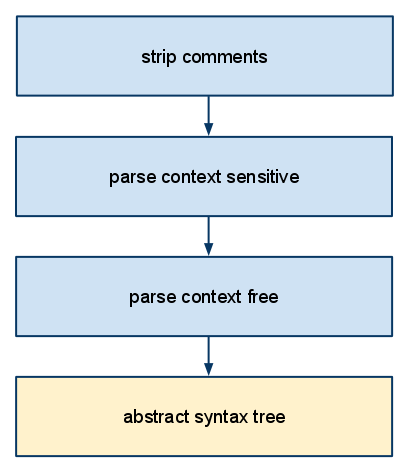
\includegraphics[width=.5\textwidth]{parser_1.png}
        \caption{Parserns olika steg}
        \label{fig:parser_steg} % Labels must come after caption!
    \end{center}
\end{figure}

Det var naturligt att dela upp parsern i tre olika steg. De tre olika stegen är skilda från varandra och vi kunde utveckla och testa dem individuellt.
Nedan följer ett exempel på parserns arbetssätt och de tre olika stegen:
\begin{lstlisting}
-- Kommentar
f x = case x of
    True -> False
    False -> True
\end{lstlisting}

Efter första steget:
\begin{lstlisting}
f x = case x of
    True -> False
    False -> True
\end{lstlisting}

Efter andra steget:
\begin{lstlisting}
f x = case x of {
    True -> False;
    False -> True
}
\end{lstlisting}

Efter det tredje steget är en AST genererad.
\begin{lstlisting}
Function("f", Lambda("x", 
    Case(VariableLookup("x"), [
        [PatternConstructor("True"), PatterConstructor("False")],
        [PatternConstructor("False"), PatterConstructor("True")],
    ])
))
\end{lstlisting}

\subsubsection{Steg 1 - Ta bort kommentarer}
Det första steget använder en parser som identifierar och tar bort kommentarer. 
Haskell har två olika kommentarsstiler, enkelradiga börjar med \emph{--} och slutar vid första radbytet och 
nästlade som kan gå över flera rader börjar med \emph{\{-} och slutar med \emph{-\}}.

\subsubsection{Steg 2 - Konvertera till kontextfri}
Det andra steget delar upp koden i dess ord och symboler samtidigt som den dekoreras med indenteringsnivåer enligt en algoritm % TODO vilken algoritm, k'a'lla
som är specifierad i haskellstandarden. Därefter användads en annan algoritm från standarden för att sätta in måsvingar och semikolon på rätt platser. % samma, vilken algoritm, TODO 
När de två algoritmerna är klara sätts koden ihop igen och skickas vidare till nästa steg.

En regel är att ett inre block inte får vara mindre indenterat än det omslutande blocket, exempelivs:
\begin{lstlisting}
case x of
    True -> ...
\end{lstlisting}
Här är \emph{True -> ...} ett inre block till \emph{case} och mer indenterat.

Ett annat exempel är:
\begin{lstlisting}
let x = 5 in x
\end{lstlisting}
Den korrekta översättningen är:
\begin{lstlisting}
let { x = 5 } in x
\end{lstlisting}
För att översätta detta korrekt kommer parsern ihåg den aktuella nästlingsnivån av "let"-uttryck och var deras repsektive "in"-uttryck befinner sig. 
Den avslutande måsvingen sätts in där ett matchande "in"-uttryck påträffas.

Ett exempel som inte översätts korrekt:
\begin{lstlisting}
[x | let x = 2]
\end{lstlisting}
Den korrekta översättningen är:
\begin{lstlisting}
[x | let { x = 2 }]
\end{lstlisting}
Men det blir:
\begin{lstlisting}
[ x | let { x = 2 ] }
\end{lstlisting}
Anledningen är att endast nästlingen av \emph{let} och \emph{in} sparas, men här finns inget \emph{in}.
För att lösa felet måste parsern hålla reda på antalet paranteser, måsvingar, hakparanteser och komman efter ett let-uttryck och när en symbol som gör det ogiltligt 
med en avslutande måsvinge påträffas sätts måsvingen in precis innan symbolen.

\subsubsection{Steg 3 - Skapa AST}
Det tredje steget är en parser för den kontextfria varianten av Haskell som den är definerad i standarden. 
Samtidigt som koden tolkas byggs en AST upp. Parsern består av en liten parser för varje grammatisk regel som är definerad i haskellstandarden 
dessa parsers kombineras ihop för att bilda den slutgiltliga parsern. Det resulterar i ett träd av parsers, en parser för hela programmet som har flera mindre parsers under sig.

Exempel:
Definitionen i haskellstandarden:
\begin{lstlisting}
gdrhs -> gd = exp [gdrhs]
rhs -> exp [where decls]
     | gdrhs [where decls]
\end{lstlisting}
Dess respektive parsers:
\begin{lstlisting}
var gdrhs = gdrhs_action(
    repeat1(gdrhs_fix_list_action(sequence(ws(gd), 
                expectws('='), ws(exp)))));

var rhs = choice(
    decl_rhs_action(sequence(expect(ws('=')), ws(exp), 
         optional(sequence(expect(ws("where")), ws(decls))))),
     sequence(ws(gdrhs), optional(sequence(expect(ws("where")), 
         ws(decls))))
);
\end{lstlisting}

Parsern använder den metod som är specifierad i Haskell 2010 \citep{haskell2010} för att lösa företrädesreglerna (precedence levels) för operatorer då denna metoden är enklare än den som är definerad i Haskell 98. 
Metoden fungerar så att den löser företrädesreglerna först efter ett uttryck har parsats till en lista med operatorer 
och uttryck, när en operator påträffas i listan slås dess företrädesnivå upp i en tabell och ett träd med 
operatorer och uttryck skapas. Sista används trädet för att generera en AST för uttrycken.

\subsubsection{JSParse}
Vi använder en modifierad version av JSParse där vi har korrigerat två fel och lagt till fler parsers. Felen vi korrigerade var i butnot-parsern och i choice-parserns cachefunktion. 
Choice-parsern cachade resultat från parsers som misslyckades och det cachade resultatet användes i senare parsers, 
vi löste det med en stackbaserad cache där cachen för en parser som misslyckas raderas.

Parsers som vi har lagt till:
\begin{enumerate}
    \item{\emph{repeatn}: en parser som upprepar en parser minst \emph{n} antal gånger}
    \item{\emph{expectws}: en parser som tillåter blanksteg och inte retunerar någon ast, är en kombination av JSParse inbyggda parsers \emph{expect} och \emph{whitespace}}
\end{enumerate}



\subsection{Interpretator}
Interpretatorns uppgift är att tolka det abstrakta syntaxträdet. Under interpreteringen används flera datastrukturer vars uppgift och struktur anges här.

\subsubsection{Thunk}
En Thunk är en avstannad beräkning, en continuation. En Thunk består av en Env och en Expression.

\begin{lstlisting}
data Thunk = Closure Env Expression
\end{lstlisting}

Haskell måste använda sig av non-strict evaluation vilket innebär att en uträkning inte får köras ifall den inte behövs. När en uträkning körs så innebär det att den resulterar i flertalet Thunks för de delar av beräkningen som ännu inte behövs. När värdet av en Thunk behövs kommer den att tvingas till en \emph{weak head normal form} (WHNF) eller en ny Thunk. Anledningen till detta är att vi på så sätt minskar användandet av rekursion vilket minskar risken att vi får ett runtime error.

\subsubsection{Weak Head Normal Form}
En WHNF är ett partiellt evaluerat uttryck. Uttrycket har blivit evaluerat så långt att vi är säkra på att det retunerar något typ av värde, alltså något som inte är undefined. Ofta innehåller en WHNF referenser till ännu icke evaluerade uttryck, om de inte gör det sägs uttrycket vara i Normal Form.

\begin{lstlisting}
data WeakHead 
    = Data Identifier [HeapPtr]
    | LambdaAbstraction Env Pattern Expression
    | DelayedApplication Env Int [Declaration] [HeapPtr]
    | Primitive
\end{lstlisting}

En Data är resultatet av att applicera en algebraisk datakonstruktor på dess argument. Argumenten ges som en lista av HeapPtr, det vill säga en lista av evaluerade eller icke evaluerade uttryck. Exemplevis resulterar Just 1 i en Data med Identifiern Just och en HeapPtr till det icke evaluerade uttrycket 1.

En LambdaAbstraction är körningsrepresentationen av en lambdafunktion, en Env är bunden till lambdafunktionen.

En DelayedApplication är ett specialfall av en LambdaAbstraction. Vi avsockrar inte Haskells funktionsdeklarationer vilket innebär att pattern matching sker även vid funktionsapplikation och inte bara i Case satser. Detta betyder att vi måste samla alla argument till en funktion innan vi kan avgöra vilket funktionsalternativ som skall användas. En vidare beskrivning finns i kapitlet Declaration.

En Primitiv är ett Javascript-värde, till exempel en integer eller en double.

\subsubsection{HeapPtr}
De flesta implementationer av Haskell använder sig av Lazy Evaluation, vilket innebär att en Thunk kommer att tvingas maximalt en gång. I vår implementation används HeapPtr som en wrapper runt en Thunk, när en HeapPtr dereferenceras kommer Thunk att tvingas till en WHNF och HeapPtr uppdateras att peka till denna. Eftersom att tvingandet av en Thunk kan resultera i en ny Thunk så tvingas thunken i en loop till dess att resultatet är en WHNF.

\begin{lstlisting}
this.dereference = function() {
    if (this.weakHead == undefined) {
        // We'll drive the execution here instead of recursing 
        // in the force method
        var continuation = this.thunk;
        while (continuation instanceof interpreter.Thunk) {
            continuation = continuation.force();
        }
        this.weakHead = continuation;
        this.thunk = null;
     }
     return this.weakHead;
};
\end{lstlisting}

\subsubsection{Env}
Env är en stack av Javascript hashes, hasharna består av en bindning mellan en Identifier och antingen en HeapPtr eller ett (Pattern, HeapPtr) par.  Den andra bindingstypen är resultatet av en VariableDeclaration där man måste utföra en pattern match för att avgöra vilken HeapPtr som hör till vilken Identifier. När man läser ut en Identifier som är bunden enligt den andra typen av binding,  kommer en pattern match att utföras och alla identifiers i det pattern som matchas kommer att bindas om som den första typen alternativt en pattern match fail inträffar och ett exception genereras.

\begin{lstlisting}
Env {
    a => ([a, b, 3], [1,2,3])
    b => ([a, b, 3], [1,2,3])
}
Env.find(a)
Env {
    a => 1
    b => 2
}
\end{lstlisting}

\subsection{Abstrakt syntaxträd} 
Vår AST representeras av javascript-objekt men dess strukturella uppbyggnad ges här av Haskells datadefinitioner.

\subsubsection{Declaration}
Den första datatypen av intresse är Declaration. En Declaration representerar en namnbindning antigen i en moduls globala definitionsområde eller i en let eller where bindning.

\begin{lstlisting}
data Declaration 
    = Variable pattern Expression
    | Data Identifier [Constructor]
    | Function Identifier [Pattern] 
        (Either [(Guard, Expression)] Expression)
\end{lstlisting}

Variable är en bindning av typen p = e där p är en Pattern och e en Expression. En Variable kan därför binda flera olika symboler på en gång. Till exempel (1:a:b:[]) = [1,2,3] binder variabeln a och b.

Function är en representation av Haskells sockrade funktionsdefinitioner. Det är möjligt att avsockra dessa till en Variable binding med hjälp av Lambda och Case men vi har valt att införa en speciell representation av funktionsdefinitioner. Till skillnad från traditionella kompilatorer så avsockras Function aldrig utan håller samma form även under interpreteringen. Tanken bakom detta är att det skall vara lättare att se sammanhanget mellan datan under körning och källkoden vilket gör det lättare att knyta samman den statiska källkoden med den dynamiska körningsdatan.

En Data definierar en algebraisk datatyp med konstruktorerna definierade som nedan
\begin{lstlisting}
data Constructor = Constructor Identifier Int
\end{lstlisting}
Värt att notera här är avsaknaden av typvariabler och typargument, detta kommer att åtgärdas när typchekaren är integrerad.

Under interpreteringen av en Declaration binds de namn (Identifiers) som definieras av Declaration till Env-objektet. Vilken typ av binding som används beror på typen av Declaration. En Variable ger en Identifier => (Pattern, Expression) bindning medan en Function eller Data ger en Identifier => Expression bindning.

\subsubsection{Expression}
En Expression är representationen av ett haskelluttryck.

\begin{lstlisting}
data Expression 
    = Constant Value
    | Lambda Pattern Expression
    | Let [Declaration] Expression
    | Case Expression [(Pattern, Expression)]
    | VariableLookup Identifier
    | Do [DoNotation]
    | List [Expression]
    | ArithmeticSequence Expression (Maybe Expression) 
                                    (Maybe Expression)
    | Primitive JavascriptFunction
\end{lstlisting}

När en Expression evalueras under en Env är resultatet antingen en Thunk (continuation, closure) eller en WHNF. Evaluering av en Constant resulterar antigen i en primitiv eller en avsockring av konstanten. I interpretatorn så är konstanta nummer, till exempel 1, egentligen en algebraisk datatyp (I\# 1\#) och denna avsockring sker först under körning. När en Lambda evalueras returneras en LambdaAbstraction med evalueringens Env bunden. En Let evalueras genom att binda dess Declarations till Env-objektet och returnera en Closure över det nya Env-objektet och Let-uttryckets Expression. En Case evalueras genom att den första Expression i tuppellistan vars Pattern matchar evalueras under den Env som resulterar från pattern matchen.
\begin{lstlisting}
this.eval = function(env) {
    var expr = new interpreter.HeapPtr(
                   new interpreter.Closure(env, this.expr));
    for (var i in this.cases) {
        var newEnv = env.derive();
        if (this.cases[i][0].match(newEnv, expr)) {
            return this.cases[i][1].eval(newEnv);
        }
    }
    throw new Error("No matching clause");
};
\end{lstlisting}
Att evaluera en VariableLookup under en Env är det samma som att leta upp en Identifier i Env-objektet.

Do, List och ArithmeticSequence är inte evaluerade direkt utan de är avsockrade och sedan evalueras det avsockrade uttrycket. Avsockringsreglerna ges i Haskell 98 standarden \citep{haskell98chap3}.

En Primitive är en wrapper runt en Javascript-funktion. Att evaluera en Primitive är det samma som att evaluera funktionen med Env som argument.

\subsubsection{Pattern}
Vi har implementerat fem stycken olika pattern matches från Haskell.
\begin{lstlisting}
data Pattern = Constructor Identifier [Pattern]
    | VariableBinding Identifier
    | Combined Identifier Pattern
    | ConstantPattern Value
    | Wildcard
\end{lstlisting}
Under en pattern match händer två saker. Dels så kontrolleras att uttrycket som matchas verkligen stämmer överens med dess pattern, dels så binds de variabler som definieras i Pattern till Env. 

En VariableBinding matchar alla uttryck och binder uttrycket till Identifier. En Constructor matchar de uttryck vars WHNF är en Data med samma Identifier (samt samma typ, detta tvingas dock av typcheckaren) och alla sub-patterns matchar Data argumenten. Combined är en sammanslagning av en VariableBinding och en annan Pattern, i källkoden så har de formen \emph{v@p}. Combined matchar de uttryck som matchar dess Pattern och binder ett matchat uttryck till Identifier. En ConstantPattern matchar de uttryck som är exakt lika med värdet. Till sist så matchar en Wildcard alla uttryck.

\subsection{Typcheckare} 
Typcheckarens uppgift är att analysera det abstrakta syntaxträdet, inferera typerna på dess olika
beståndsdelar och avgöra om sättet på vilket de används och interagerar med
andra beståndsdelar är konsekvent. Om så inte är fallet sägs programmet ha
typfel.

\subsubsection{Haskells typsystem}
Jämfört med mer konventionella språk (C, C++, Java etc) skiljer sig Haskell
och övriga statiskt typade funktionella språk på flera sätt. I de senare
medges i många fall att programmeraren själv inte behöver ge explicita
typdeklarationer för variabler och funktioner. Istället arbetar typcheckaren
med en process där kriterier samlas in för varje enskild beståndsdel och
sedan utifrån detta försöker finna en så allmän typ som möjligt eller om
detta inte är möjligt; meddela programmeraren om typfel. Denna process
kallas typinferens.

Typinferens möjliggör även för polymorfiska typer vilket innebär att
typcheckaren alltid försöker hålla en typ så allmän som möjligt. Om
exempelvis en funktion inte är beroende av funktionalitet associerad med en
specifik typ hos något av sina argument kan data av alla typer användas som
argumentet.

Utöver polymorfiska typer stödjer Haskell typklasser som gör överlagring av
funktioner möjligt. Typklasser är väldigt centralt i Haskell och ändrar
typcheckarens arbetssätt markant jämfört med liknande språk.

\subsubsection{Kinds}
Kinds kan liknas vid en motsvarighet till typer för typkonstruktorer. * (uttalas ``stjärna'', eng. ``star'') representerar enkla (nullary) typer som Integer och Integer -> Bool medan komplexa typer som tar argument representeras med applicering av kinds k1 -> k1, exempelvis Maybe Bool.

\begin{lstlisting}
data Kind = Star
          | Kfun Kind Kind
\end{lstlisting}

\subsubsection{Typer}
De datastrukturer som typcheckaren använder internt för att representera typer kan delas in i typvariabler som representerar 

För att kunna arbeta på en hög abstraktionsnivå har typcheckaren sin egen
interna representation av typer.

\begin{lstlisting}
data Type = TVar Id Kind
          | TAp Type Type
          | TCon Id Kind
          | TGen Int     
\end{lstlisting}

TVar representerar typvariabler. Dessa har namn som vanligtvis tilldelas internt i typcheckaren. TAp representerar applicering av typer och TCon representerar typkonstruktorer för konkreta typer. TGen representerar
generiska typer och används enbart i samband med kvantifiering av
typer internt i typcheckaren

Att konstruera en typ med den här notationen är enkelt. Typen \emph{[a] ->
Integer} som är typen för standardfunktionen length i Haskell beskrivs med
\begin{lstlisting}
(TAp
  (TAp
    (TCon "(->)" (Kfun Star (Kfun Star Star)))
  (TAp
      (TCon "[]" (Kfun Star Star))
      (TVar "a" Star)))
  (TCon "Integer" Star))
\end{lstlisting}

\subsubsection{Substitueringar}
Substitueringar är mappningar \emph{typvariabel -> typ} och används av typcheckaren
för att hålla typer uppdaterade efterhand som den får ny
information. Typcheckaren innehåller flera funktioner som opererar på
substitutioner, bland annat komponering och sammanfogning av
substitutioner. \emph{Unifiering} är processen att finna en substituering som gör två typer ekvivalenta. Om unifiering inte är möjligt
betyder det att det finns typfel.

\subsubsection{Typklasser}
Typklasser är en form av ad-hoc polymorfism som används flitigt i
Haskell. Faktum är att de är så fundamentala i Haskell att de får en central
roll i typcheckningsprocessen. Deras främsta funktion är att möjliggöra funktionsöverlagring beroende på typer på argument och förväntad returtyp.

För att hålla reda på vilka typklasser en typ tillhör används predikat:
\begin{lstlisting}
data Pred = Pred Id Type
\end{lstlisting}
Ett predikat \emph{Pred className type} säger att typen \emph{type} tillhör typklassen \emph{className}.

Ofta består typer av flera sammansatta enklare typer där olika typer kan tillhöra olika typklasser. För att modellera detta används kvalifierade typer:
\begin{lstlisting}
data Qual = Qual [Pred] Type
\end{lstlisting}

Den kvalifierade typen \emph{Monad m => m a} modelleras som:
\begin{lstlisting}
(Qual
  [ Pred "Monad" (TVar "m" (Kfun Star Star)) ]
  (TAp
    (TVar "m" (Kfun Star Star))
    (TVar "a" Star)))
\end{lstlisting}

För att modellera de hela typscheman som typcheckaren får in från användaren används datatypen \emph{Scheme}.
\begin{lstlisting}
data Scheme = Scheme [Kind] Qual
\end{lstlisting}
Eftersom typvariabler (\emph{TVar id kind}) endast skapas internt i typcheckaren så representeras här alla generiska typer med \emph{TGen n} där \emph{n} helt enkelt anger att det är den \emph{n}:te generiska typen i typschemat och dess kind finns lagrat på position \emph{n} i \emph{[Kind]}

För att representera det tidigare exemplet på detta sätt byter vi ut alla identiska förekomster av \emph{TVar id kind} mot identiska \emph{TGen i}:
\begin{lstlisting}
(Scheme
  [Kfun Star Star, Star]
  (Qual
    [Pred "Monad" (TGen 0)]
    (TAp
      (TGen 0)
      (TGen 1))))
\end{lstlisting}

För att hålla reda på vilka typklasser och instanser som finns används datatypen \emph{Klass} (\emph{class} är ett reserverat ord i JavaScript) som representerar enskilda typklasser och deras instanser samt datatypen \emph{KlassEnvironment} som representerar den totala klassmiljön.

\subsubsection{Typinferens}
Typinferens är den sammanfogande delen av typcheckningsprocessen och går ut på att typcheckaren traverserar abstrakta syntaxträdet och samlar de kriterier som måste vara uppfyllda för att programmet ska vara korrekt.

Eftersom en variabels exakta typ inte är helt fastställd förrän typcheckningsprocessen är färdig görs istället efterhand antaganden om dess typ. För att modellera ett sådant antagande används datatypen \emph{Assump}:
\begin{lstlisting}
data Assump = Assump Id Scheme
\end{lstlisting}

Typinferensen är beroende av att en antal komponenter finns tillgängliga. Dessa är registret över typklasser och instanser \emph{KlassEnv}, listan över antagna variabeltyper, en generator för unika typvariabler med funktionen \emph{newTVar} och substitueringas \emph{Subst}. Dessa samlas i objektet \emph{Environment} som skickas som argument till funktionerna i typinferensen. 
För att bättre illustrera hur typinfereringsprocessen går till ger vi ett konkret exempel. Koden nedan visar hur typinferering av \emph{if}-uttryck går till. Eftersom vårt projekt avsockrar \emph{if}-uttryck till \emph{case} använder det inte exempelkoden men då den på ett bra sätt illustrerar konceptett väljer vi här ändå att använda den:

\begin{lstlisting}
ast.If.prototype.infer = function(env) {
  var b = this.condExpr.infer(env);
  env.unify(
    b.type,
    new typechecker.TCon(``Bool'', new typechecker.Star()));
  var te = this.thenExpr.infer(env);
  val ee = this.elseExpr.infer(env);
  env.unify(te.type, ee.type);
  return {
    preds: te.preds.concat(ee.preds),
    type: te.type
  };
};
\end{lstlisting}
Först infereras typen på vilkoret. Detta unifieras med typen \emph{Bool} på raden under. Sedan infereras typerna på \emph{then}- respektive \emph{else}-delarna och då dessa måste vara va samma typ unifieras deras typer. Till sist returneras de insamlade predikaten från både \emph{then}- och \emph{else}-delarna tillsammans med den unifierade typen.

Av detta exempel kan ett antal slutsatser dras. Typinfereringen sker rekursivt från sammansatta uttryck ner till de alla enklaste literalerna. Att misslyckande av unifiering betyder typfel innebär att inferera-unifiera-cykeln har en roll liknande den infer-check har vid typcheckning i exempelvis C.

\subsubsection{Defaulting}
Ofta förekommer situationer där tvetydigheter gör att typcheckaren inte kan bestämma en typ. För att förenkla för programmeraren finns därför förbestämda standardtyper att använda i dessa situationer för en del inbyggda typer. Detta användande av förbestämda standartyper kallas för defaulting.

\subsection{HIJi}

HIJi är ett program som ger användaren ett GHCi-liknande användargränssnitt till haskelltolken i webläsaren. 
HIJi tar indata genom att funktioner skrivs in i HIJi som sedan tolkas av parsern och i sin tur bygger upp det abstrakta syntaxträdet. Därefter evalueras uttrycket av interpretern och resultatet blir synligt i HIJi.

HIJi har stöd för att ladda externa moduler. Det görs genom att skriva :l \emph{namn-på-modul}. Användaren får då tillgång till alla de funktioner som är skrivna i den modulen. Modulerna måste vara placerade på servern som HIJi laddades ifrån. Modulerna kan ej laddas direkt från användarens hårddisk på grund av att javascript av säkerhetsskäl ej har skriv och läsrättigheter av användarens filsystem. HIJi har även en förladdad modul, Prelude, som innehåller en delmängd av de funktioner som finns i GHCis motsvarighet. 

Den indata som användaren skriver till HIJi sparas i ett objekt för att hantera historiken. För att bläddra i historiken används piltangenterna Upp och Ner. Hela historik-objektet sparas även i en kaka som ett JSON-objekt. Av detta skäl är det möjligt att få tillgång till historiken när en ny session av webbläsaren startas.

\begin{figure}[H]
    \begin{center}
        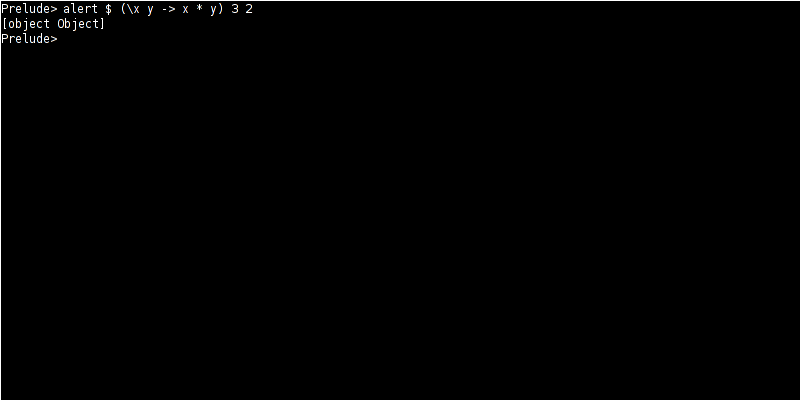
\includegraphics[width=1\textwidth]{hiji_screen3.png}
        \caption{HIJi användargränssnitt}
        \label{fig:hiji} % Labels must come after caption!
    \end{center}
\end{figure}

Figur \ref{fig:hiji} visar hur HIJi ser ut. De första raderna visar, precis som i GHCi, vilka moduler som för närvarande är laddade. I det här exemplet är den förladdade modulen Prelude laddad. Därefter följer en kommandotolk där användaren fritt kan skriva in egna funktioner. I figuren är en lambda-funktion inskriven.

HIJi är skapat för att likna GHCi i så stor utsträckning som möjligt.
Genom att efterlikna GHCi kommer användare känna igen sig när de tar steget från HIJi till GHCi. Det blir för dem ett naturligt steg och kortar inlärningströskeln. Även för haskellprogrammerare som är vana användare av GHCi blir det lättare att använda sig av HIJi, de behöver inte fundera hur verktyget ska användas.

    \newpage
    \section{Diskussion}
Vi har skapat en javascriptapplikation som kan parsa, typchecka och interpretera stora delar av Haskell 98. Det som saknas är fullständigt stöd för typklasser där stödet endast finns i typcheckaren och parsern men fortfarande behöver implementeras i interpretatorn. Detta handlar främst om förmågan att välja rätt instanser av typklasser vid applicering av överlagrade funktioner.

Sett till planeringen har vi lyckats uppfylla alla milstolpar utom typklasser, dock inte enligt den ordning och tidsplan som ursprungligen planerades. 
Vi insåg att det var enklast att utveckla parsern, typcheckaren och interpertatorn parallelt och bestämma individuellt vad som skulle implementeras och i 
vilken ordning för att senare, oftast en gång i veckan, samordna och implementera det som behövdes i flera delar.

Vi har inte implementerat NPlusK-pattern i parsern och då de är borttagna i Haskell 2010 \citep{haskell2010} känner vi att det inte behövs.

\subsection{Val av språk för implementering}
Tidigt i planeringen tvingades vi välja vilket språk vår implementation skulle
bestå av. Det första alternativet var att först skriva en kompilator för att
kompilera Haskell till JavaScript. Därefter skulle så kallad boot-strapping
tillämpas där kompilatorn används för att kompilera sig själv till
JavaScript. Eftersom det redan finns parsers och typcheckare för Haskell
skrivna i Haskell skulle projektet mestadels handla om att finna en lämplig
målrepresentation för Haskell i Javascript-kod och sedan implementering av en
kodgenerator för denna. Haskells statiska typcheckning och referentiella
transparens skulle också förenkla verifiering av projektets komponenter.

Dock finns även en del nackdelar med en sådan implementation. Utan särskilda
optimeringar i kompilatorn skulle en målrepresentation nödvändigtvis innehålla
strukturer liknande dem man finner i en interpreterare för ett lat evaluerat
språk. Det är ett rimligt antagande att sådana optimeringar tack vare graden
på sin komplexitet vore alltför stora för att genomföra i en kurs som
denna. Därför anser vi att denna typ av implementation lämpar sig bäst inom
ramarna för ett existerande kompilatorprojekt såsom GHC där nödvändiga optimeringar redan finns innbyggda.

Det andra alternativet var att skriva allt i Javascript och detta är den
implementationsstrategi som vi till slut bestämde oss för. Den största
fördelen med en sådan implementation är att integrering med annan
Javascript-kod blir enkel. Det första alternativet skulle däremot kräva ett
särskilt integrationslager för att få samma möjligheter.

Det andra alternativet hade också fördelen att en stor del av vår projekts potentiella användare redan har viss erfarenhet av Javascript och liknande språk och att användande av vårt bibliotek därför blir enklare för dessa än vad motsvarande haskellimplementation skulle bli. Eftersom detta alternativ krävde att vi själva implementerar parser, typcheckare och interpreterare ansåg vi också att det gav oss större möjligheter till lärande. 

\subsection{Framtida förbättringar}

Syftet med projektet, att skapa en fungerande Haskelltolk i javascript, har vi lyckats implementera om man tar hänsyn till de avgränsningar som är uppsatta. Dock om man ser till motivationen bakom projektet, att vår Haskelltolk ska kunna användas som grund för att skapa en webbaserad interaktiv läroplattform, så finns det fortfarande mycket kvar att utveckla. Framförallt handlar det om att göra Haskelltolken och HIJi mer lättanvänd för nybörjare inom funktionell programmering.

I parsern har vi identifierat två förbättringsmöjligheter. För det första, bättre felmeddelanden
Hjälpsamma och förklarande felmeddelanden är en viktigt del av ett utvecklingsverktyg och det generars för tillfället inte av parsern. 
Om parsern stöter på ett fel rapporterar den endast att ett fel har inträffat och avslutar parsningsprocessen. 
Att förbättra dessa felmeddelanden med exempelivs rad- och kolumnnummer och specifik information om vad för fel som har inträffat skulle göra parsern mer användbar.
För att implentera detta behöver man kombinera steg 1 och 2 i parsningen för att rad- och kolumn-nummer ska bevaras korrekt då borttagning av nästlade kommentarer kan påverka dessa.
JSParse behöver modifieras så att det rapporterar var ett fel uppstod och i vilken parser.

För det andra, konverteringen av icke kontextfri Haskellkod till kontextfri kan förbättras 
för att klara av att expandera måsvingar i \emph{[x | let x = 5]}. 
För att klara av detta behövs en parser som räknar antal måsvingar, paranteser, 
komman och hakparanteser efter \emph{let} och avgöra när det är korrekt att sätta in avslutande måsvingar.

Även i HIJi finns det förbättringar att göra.
Det som framförallt behöver utvecklas är, för det första, erbjuda en interaktiv tutorial där användaren får instruktioner vad som ska skrivas in i HIJi. Om användaren skriver in rätt uttryck fortsätter tutorialen till nästa nivå.
För det andra, visa typinformation från funktioner genom att hålla musen över funktionsnamnet.
Och tillsist, kunna stega igenom ett program eller funktion för att kunna se vad som händer i varje evalutionssteg. 

    \newpage
    \section{Slutsatser}

\subsection{Framtida förbättringar}


\subsubsection{Parser}
Hjälpsamma och förklarande felmeddelanden är en viktigt del av ett utvecklingsverktyg och det generars för tillfället inte av parsern. 
Om parsern stöter på ett fel rapporterar den endast att ett fel har inträffat och avslutar parsningsprocessen. 
Att förbättra dessa felmeddelanden med exempelivs rad- och kolumnnummer skulle göra parsern mer användbar.

För att implentera detta behöver man kombinera steg 1 och 2 i parsningen för att rad- och kolumn-nummer ska bevaras korrekt då borttagning av nästlade kommentarer kan påverka dessa.

Konverteringen av icke kontextfri Haskellkod till kontextfri kan förbättras 
för att klara av att expandera måsvingar i \empth{[x | let x = 5]}, 
för att klara av detta behövs en parser som räknar antal måsvingar, paranteser, 
komman och hakparanteser efter \emph{let} och avgöra när det är korrekt att sätta in avslutande måsvingar.

\subsubsection{HIJi}
HIJi är tänkt som ett webbaserat verktyg för nybörjare att komma igång med funktionell programmering. Ur det perspektivet når HIJi ännu inte upp till de krav som en nybörjare kan förvänta sig. Avsaknaden av interaktivitet är den i dagsläget största nackdelen. Här är de förbättringar som vi anser vara nödvändiga för att nybörjare ska kunna använda sig utav HIJi.

Erbjuda en interaktiv tutorial där användaren får instruktioner vad som ska skrivas in i HIJi. Om använaren skriver in rätt uttryck fortsätter tutorialen till nästa nivå.

Få ut typinformation ur funktioner genom att hålla musen över funktionsnamnet. 

    \newpage
    

    % källor 
    \bibliographystyle{plainnat}
    \bibliography{kallor} 
    
    \end{document}
